\documentclass{l4proj}

\usepackage{url}
\usepackage{fancyvrb}
\usepackage[final]{pdfpages}
\usepackage{hyperref}
\usepackage{fancyvrb}
\usepackage{float}
\usepackage{multirow}
\usepackage{graphicx}
\usepackage{amsmath}
\usepackage{MnSymbol}
\usepackage{wasysym}
\usepackage{mathtools}
\usepackage{subcaption}
\usepackage{relsize}
\usepackage{algorithm}
\usepackage[noend]{algpseudocode}

\hypersetup{
    colorlinks,
    citecolor=black,
    filecolor=black,
    linkcolor=black,
    urlcolor=black
}

\makeatletter
\def\BState{\State\hskip-\ALG@thistlm}
\makeatother

\begin{document}
\title{Implementations of Advanced K-Means Clustering Algorithms \\ for Spark/MLlib}
\author{Ivan Kyosev}
\date{March 21, 2017}
\maketitle

\begin{abstract}
Apache Spark is a fast and general engine for large-scale data processing. It emphasizes speed, ease of use and generality in regards to working with Big Data. Its feature-set provides an alternative to the popular Hadoop MapReduce software framework, displaying a noticeable performance improvement. One of Spark's many components is MLlib. It is a machine learning library built on top of the core features of Spark and provides implementations for a variety of popular machine learning algorithms, written in a way meant to support scalability when operating on big data sets.

This paper presents a proposed extension to the MLlib component of Apache Spark in the form of additional K-Means Clustering algorithms that the library does not currently support. K-Means clustering is a method of vector quantization, originally from signal processing, that is popular for cluster analysis in data mining. A thorough analysis of the performance of the newly created algorithms and the relative quality of the produced data models is also conducted.
\end{abstract}

\educationalconsent

\tableofcontents

\chapter{Introduction}
\label{intro}
\pagenumbering{arabic}

Machine learning is an increasingly popular and relevant part of modern day systems looking to extract knowledge and value from the world around them. It refers to an approach to computation, where applications can learn without being explicitly programmed. These kinds of apps can analyze a provided sample of data and make predictions or decisions, based on some form of discovered pattern or correlation between the individual elements of the input set.

By being able to take rational choices, through examining the surrounding environment, systems that employ machine learning have become a central component of artificial intelligence. Because these system adapt their behavior based on new ``experiences'' they are utilized in a wide range of computing tasks, where developing explicit algorithms is not feasible. Such examples include solving problems in speech recognition, vision and robotics.

These machine learning algorithms are typically classified into three different categories based on the nature of the data they are learning from and the feedback of information for each input item:

\begin{itemize}
\item Supervised learning - in this case a program presented with a particular input set of data is also given the desired output, with the end goal of having the machine learn a mapping function from inputs to outputs
\item Unsupervised learning - here the elements of the input data set are not provided with a desired output value in pairs, so the system is left on its own to find structure in its input
\item Reinforcement learning - this refers to the idea of having an program interact with a dynamic environment, where it is attempting to achieve a certain goal. Along with every action, the program is also provided with positive or negative feedback, depending on whether the action aided in achieving the goal or not. 
\end{itemize}

Many of these machine learning algorithms have a similar underlying approach to their implementation. Input training data with some unknown probability distribution is presented and the program has to construct a model that allows it to extract meaning from the data and make sufficiently accurate predictions for instances that have not been encountered yet. This is generally achieved by defining a loss function and adjusting the model in attempts to minimize this loss with respect to the inputs -- effectively an optimization problem.

It is clear that machine learning algorithms heavily depend on the availability of input data in order to optimize their models to more accurately reflect the state of the real world. Therefore the quantity of supplied input data begins to have a significant impact on the quality of the output produced by application relying on machine learning. With the advent of big data and technologies meant to enable fast and reliable processing of big data, these algorithms can now make use of vast amounts of information, enabling them to create more accurate and valuable results. Examples of big data processing frameworks include Hadoop and Apache Spark.

The Apache Spark project in particular includes a component called MLlib. MLlib is a machine learning library built on top of the core features of Spark. It provides implementations for a variety of popular machine learning algorithms, all of which are written in a way meant to support horizontal scalability\footnote{Horizontal scaling refers to the scaling of a system by adding more parallel, similar in performance nodes. It is directly contrasted by vertical scaling where additional resources are added to the one node of a system.} when operating on big data sets.

\section{Aims}

The aim of this project is to create an extension to the MLlib component of Apache Spark, by developing implementations for a variety of K-Means clustering algorithms that the framework does not currently support. The newly introduced algorithms also need to be evaluated and contrasted with the ones already provided by Spark.

K-Means clustering is an example of an unsupervised machine learning algorithm. It is a method of vector quantization\footnote{Quantization is the process of mapping a large set of input values to a smaller set.}, that originated from signal processing. Its primary purpose is to group a collection of \texttt{N} data points into \texttt{K} distinct clusters. There is a variety of algorithms that produce the end result of grouping data points into \texttt{K} clusters, with varying levels of speed and accuracy. The ones that this project aims to implement as part of Spark could deliver a desired performance improvement with minimal loss in quality.

\section{Report outline}

The remainder of this report will focus on the mathematics underlying each of the considered K-Means clustering algorithms as well as the challenges of implementing them in a scalable fashion under Spark:
\begin{itemize}
\item \textbf{Chapter~\ref{spark}} covers the data processing model provided by Apache Spark and its machine learning library MLlib
\item \textbf{Chapter~\ref{kmeans}} explains the most common used versions of K-Means Clustering algorithms
\item \textbf{Chapter~\ref{previous}} discusses the approach taken by Spark's developers to create the current clustering API
\item \textbf{Chapter~\ref{propose}} outlines the proposed algorithms to be implemented as part of Apache Sparks, along with their benefits and challenges
\item \textbf{Chapter~\ref{online}} details two different approaches to the implementation of Lloyd's Online K-Means Clustering algorithm
\item \textbf{Chapter~\ref{art}} presents a version of K-Means using Adaptive Resonance Theory and its implementation
\item \textbf{Chapter~\ref{som}} presents the implementation of a  a K-Means Clustering algorithm using Self-Organizing Maps
\item \textbf{Chapter~\ref{eval}} covers a variety of ways to evaluate both the performance of the presented algorithms and the quality of the data models they produce
\item \textbf{Chapter~\ref{conclusion}} Concludes this report with a reflection on the whole project
\end{itemize}

%==============================================================================

\chapter{Introduction to Apache Spark and MLlib}
\label{spark}
\section{Apache Spark}

A new big data processing paradigm in the form of cluster computing has become widely popular in recent years. It is a model where data-parallel computations are executed on clusters of unreliable machines by systems that provide scheduling, fault tolerance and load balancing\cite{Spark}. Hadoop MapReduce was the first software framework to implement these principles\cite{MapReduce}, with systems like Dryad and Map-Reduce-Merge generalizing the supported types of data flows. These system achieve fault tolerance and scalability by supplying the user with a means of expressing computation as an acyclic data flow graph which passes the input data through a set of operations. This enables the underlying system to handle any occurring faults as well as scheduling without any user interaction.

Apache Spark is one of the latest big data processing frameworks which implements the cluster computing model. One of its primary advantages over Hadoop is that it can perform in-memory data processing, while Map-Reduce persists all outputs back to disk after a map or reduce action. This extends the scope of problems which can be solved efficiently by Spark to also include applications that reuse a working set of data across multiple parallel operations. It is impractical to implement these kinds of apps under Hadoop as between each iteration of an algorithm over the working set, the job must reload the data from disk, causing unnecessary overhead, resulting in degraded performance. Examples include iterative jobs and interactive analysis\cite{Spark}.

Due to its differences in design philosophy, users of the Spark framework have reported a 100x speed increase in certain work loads, versus a similar MapReduce solution, as well as a 10x faster execution on disk\cite{webSpark}. This performance improvement, however, results in the system requiring more RAM to carry out its operations.

The core components of Spark are implemented in Scala - a statically typed functional programming language that runs on top of the Java Virtual Machine. It also includes object-oriented features and supports Java interoperability thanks to its JVM roots -- this allows Spark to easily interact with Java based systems such as HDFS. In addition to Scala the framework also export an API available in Java, Python and R.

Spark can also be used interactively from a modified version of the Scala interpreter. This method provides full access to the API, allowing a user to define variables, functions, classes and run parallel jobs on a computer cluster. Spark is possibly the first system that allows a general-purpose programming language to be used interactively to process large data sets on a cluster\cite{Spark}.

\section{Resilient Distributed Datasets}

To achieve its goals, Spark introduces an abstraction called resilient distributed datasets -- RDDs. They are a parallel, fault-tolerant data structure that lets users explicitly persist intermediate results in memory, control their partitioning to optimize data placement, and manipulate them using a rich set of operations\cite{RDD}. The RDD API is the primary way of expressing computation on big data sets in Apache Spark.

\subsection{Basics of the RDD API}

An RDD is a read-only partitioned collection of records. It supports a series of methods that resemble operations, available to most collections in a functional programming language\footnote{Despite the nature of the RDD based API, code written in Spark does not need to adhere to the principles of pure functional programing.}. RDDs can only be created through deterministic operations on either data in stable storage or other RDDS. These kind of functions are known as transformations -- examples include \textit{map}, \textit{filter}, \textit{flatMap} and others. Transformations are lazy\footnote{A lazy function is not evaluated when it is called, but rather when something else tries to access its result.} operations that define a new RDD, which is typically the result of applying the same function to every data item in the source RDD -- making Spark ideal for batch processing. By chaining together several of these transformations a user can define a directed acyclic graph (DAC) of operations the data needs to pass through (achieved in a parallel fashion).

Along with transformations, the RDD API also supports actions. These are operations that return a value to the application or export data to a storage system. Examples of actions include - \textit{count}, \textit{collect}, \textit{reduce} and others. Typically a user would define a DAC of transformations to be performed on some data source, these operations would then not be executed until an action is invoked, at which point the result of all transformations in the DAC is evaluated along with the specified action at the end. If there is a large sequence of transformations within the DAC of an RDD, that will be operated on in the end by multiple different actions (branching towards a later point in the DAC), a developer might choose to checkpoint an intermediate stage of the RDD, so that Spark does not need to recompute every operation applied to that RDD.

\begin{table}[H]
\label{Actions and Transformations}
\caption{Transformations and actions available on RDDs in Spark.}
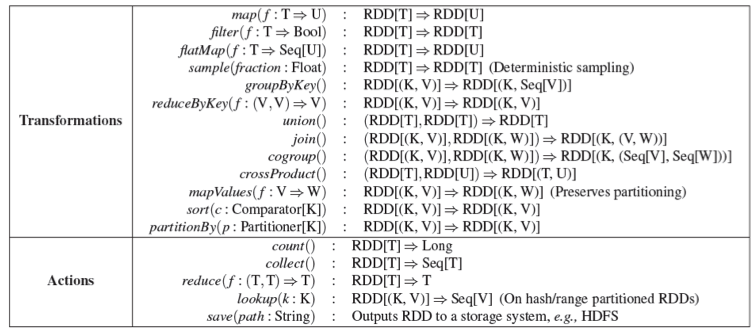
\includegraphics[width=1.0\textwidth]{images/spark-trans-action-edited}
\end{table}

\subsection{RDD fault-tolerance}

To begin the processing of an RDD, the individual data partitions (making up the source used to create the RDD -- typically a file in HDFS), are sent to different nodes in the computing cluster where the user defined DAC of operations is executed simultaneously for each partition (if the system could afford to allocate enough resources for a one-to-one mapping of partitions to cluster nodes). In a large scale distributed system, however, failure of individual hardware components is to be expected. When one of the clusters fails, while processing an RDD partition, Spark is able to reconstruct the lost data without notifying the user.

Because RDDs provide an interface based on transformations (e.g. map, flatMap) that apply the same operations to many data items, they can efficiently provide fault-tolerance by logging the transformations used to build a dataset rather than the actual data (although checkpointing RDDs can have its advantages as previously mentioned). This log of operations is also known as the lineage of the RDD. Thus if a partition of an RDD is lost, the RDD has enough information about how it was derived from other RDDs to recompute just the missing partition\cite{RDD}. Therefore lost data can be quickly recovered without the need for costly replication.

The lineage of an RDD is a powerful property, since it ensures that a program cannot reference an RDD that it cannot reconstruct after failure -- it can always recompute all partitions from data in stable storage.

\subsection{RDD representation}

The Apache Spark framework provides a graph-based representation of RDDs where each dataset has a common interface, exposing five pieces of information:

\begin{itemize}
\renewcommand{\labelitemi}{\scriptsize$\blacksquare$}
\item a set of partitions, which are atomic pieces of the dataset
\item a set of dependencies on parent RDDs
\item a function for computing the dataset based on its parents
\item metadata about its partition scheme
\item metadata about its data placement
\end{itemize}

An RDD representing an HDFS file, for example, has as many partitions as the file has blocks and knows on which machine each block is on. If a map transformation were to be applied on this RDD, the resulting dataset would have the same partitions, but the map function would be applied on the parent's data when computing its elements.

An important aspect of this common interface is the representation of dependencies between RDDs. They are classified into two types: \textit{narrow} dependencies, where each partition of the parent RDD is used by at most one partition of the child RDD, and \textit{wide} dependencies where multiple child partitions may depend on a single parent partition\cite{RDD}. The \textit{map} operation would be an example of a narrow dependency, where as \textit{groupByKey} would result in a wide dependency.

The distinction between these two forms of dependencies has two primary implications. First, narrow dependencies allow for pipelined execution on one cluster node. This means that multiple successive operations resulting in narrow dependencies can be carried out on an RDD partition in the same computing cluster, without needing to move data between cluster nodes. Wide dependencies, however, require that data from all parent partitions to be available and to be shuffled across the nodes of the cluster. Second, narrow dependencies allow for a more efficient recovery from failure, as only the lost partitions need to be recomputed -- this can also be done in parallel on different processing nodes. When there are wide dependencies in the lineage graph of an RDD, however, a single failed node could loose information derived from all parent partitions, requiring a full re-execution of all transformations in the DAC, operating on the RDD.

\begin{figure}[H]
\label{RDD dependencies}
\caption{Examples  of  narrow  and  wide  dependencies.  Each box is an RDD, with partitions shown as shaded rectangles.}
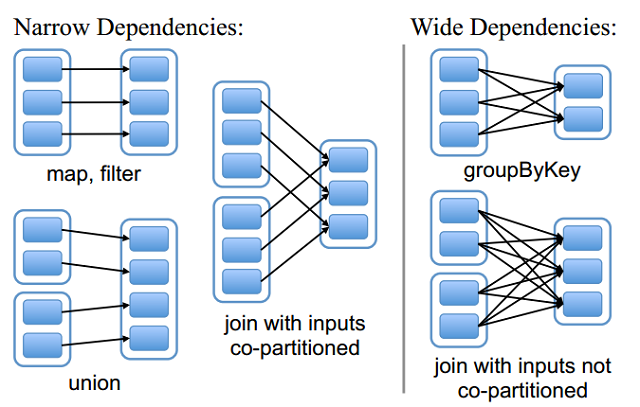
\includegraphics[width=1.0\textwidth]{images/rdd_dependency}
\end{figure}

\section{Shared Variables}

When invoking transformations on an RDD -- such as \textit{map} and \textit{filter}, developers pass closures (functions) to Spark. Similar to functional programming these closures can refer to any variable in the scope where they are created. Once Spark begins the execution of those transformations on a worker node, the referenced local variables are copied to the worker. However, Spark also allows programmers to create two restricted types of shared variables to support common usage patterns\cite{Spark}.

If a Spark program contains a large read-only piece of data that is used in multiple parallel operations, it is preferable to distribute it to the workers only once, as opposed to including it with each closure. This is accomplished by creating a ``broadcast variable'' object which acts as a wrapper for the desired value. It ensures that it is only copied once to each worker, thus reducing network traffic and improving performance.

The second type of shared variables provided by Spark are known as ``accumulators''. Workers can only ``add'' to these variables by using an associative operation, and their value can only be read by the driver program. They enable easy implementations of counters (similar to MapReduce) and provide a more imperative syntax for parallel sums. Accumulators can be defined for any data type that has a ``zero value'' and an ``add'' operation.

\section{Spark Streaming}

In addition to its base API, Spark also provides a solution for developing applications based on sacalble, high-throughput, fault-tolerant stream processing of live data. This is achieved thanks to Spark Streaming - a system that allows data to be ingested from many sources like Kafka, Flume, Kinesis, or TCP sockets, and later processed using complex algorithms expressed with high-level functions.

Once a Spark program defines a input data source, Spark Streaming can receive a live data stream from the specified source, which is then divided into batches that are later processed by the Spark engine. The primary abstraction that implements this operation is the \textit{discretized stream} or \textit{DStream}\cite{DStream}. It is represented internally as a sequence of RDDs.

Once a DStream has been created from a specified live data source (e.g. Kafka, an HDFS directory, whose content is being simultaneously altered by a different application, etc.) or alternatively from a different DStream, it begins to store or log any new information it has received. A program utilizing Spark Streaming needs to also specify a batch interval to the streaming context -- used to configure all DStreams for that application. At the end of every interval the DStream produces an RDD, containing all the data output from the specified source, since the start of the interval. The resulting RDDs are then processed by the remaining application logic -- various transformations and actions. Finally, the batch interval must be set based on the latency requirements of  the application and the available cluster resources.

\section{MLlib}

The Apache Spark project also includes a distributed machine learning library, built on top of Spark's core features -- MLlib. MLlib provides efficient functionality for a wide range of learning settings and includes several underlying statistical, optimization,
and linear algebra primitives. It exploits the benefits of Spark's fault-tolerant, parallel big data processing paradigm to deliver fast and scalable implementations of standard learning algorithms for common learning settings including:  classification, regression, collaborative filtering, clustering, and dimensionality reduction\cite{MLlib}.

MLlib also inter-operates well with Spark's other major components. Thanks to Spark SQL\cite{SQL} developers can more easily designate their prior storage solutions as the data source of the desired machine learning algorithms. Spark Streaming is also used by MLlib to enable applications to learn from real-time online streamed data, however, this is only supported by certain algorithms.

%==============================================================================

\chapter{K-Means Clustering}
\label{kmeans}

A long time pursuit in the field of artificial intelligence and machine learning has been to grant machines the ability to differentiate between discrete objects with similar or vastly different properties and to be able to identify and classify them. At a high level, an AI would need to be able to examine the features of an object, which has not been previously encountered and create an internal, digital representation of it. Then the machine would need to perform a computation on that model to extract meaning from it and predict the nature of the object, without human input - i.e. explicitly providing a label.

Recent developments in image processing and robotics have had a great impact on the field of machine learning, in regards to allowing systems that employ these practices to interact more directly in the real world. The aim of this paper, however, is not to cover techniques for creating a mapping from real world objects to internal, machine friendly representations of their properties, but rather to outline the implementation of algorithms for operating on said representations -- focusing on cluster analysis.

Cluster analysis is concerned with the task of grouping a set of objects in a way, such that objects in the same group (known as a cluster) are more similar to each other than those in other groups\cite{MLIntro}. It is commonly used in statistical data analysis as well as data mining. Along with machine learning, cluster analysis has applications in other fields such as pattern recognition, information retrieval, biometrics and others.

In cluster analysis, different approaches to the problem of groping data together can vary greatly -- algorithms can differ in their notation regarding what constitutes a cluster, as well as how to find them. Popular definitions of clusters include: groups with small distances between the individual cluster members, dense areas of the data space or specific statistical distributions. Given a way of evaluating the quality of a particular assignment of individuals to groups, clustering can also be described as an optimization problem, were we are trying to maximize that value.

K-Means clustering is an examples of cluster analysis with a centroid-based model\cite{TopTen}. It was originally used in signal processing as a method for vector quantization. K-Means functions by partitioning \texttt{N} observable objects into \texttt{K} distinct clusters, where every object belongs to the cluster with the nearest mean  -- here these observations will only take the form of N-dimensional data points. The actual clusters are represented as a central vector (N-dimensional point), which does not necessarily belong to the input set.

\begin{figure}[H]
\label{basic clusters}
\centering
\begin{subfigure}{.5\textwidth}
  \centering
  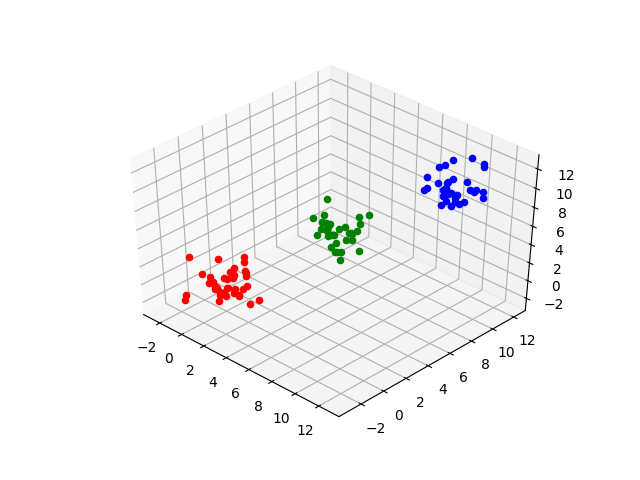
\includegraphics[width=1.2\linewidth]{images/figure_1}
  \label{fig:sub1}
\end{subfigure}%
\begin{subfigure}{.5\textwidth}
  \centering
  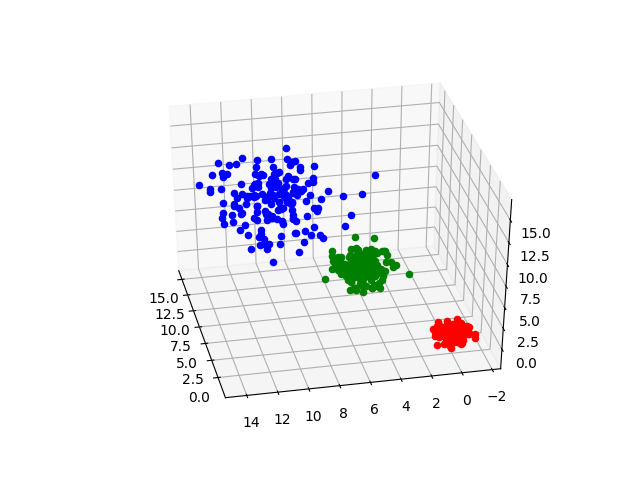
\includegraphics[width=1.2\linewidth]{images/figure_2}
  \label{fig:sub2}
\end{subfigure}
\caption{Examples of three distinct clusters in 3 dimensional space}
\label{fig:test}
\end{figure}

When the number of centroids \texttt{K} is fixed, K-Means clustering provides a formal definition of an optimization problem: find the \texttt{K} cluster centers and assign the input data points to the nearest center, such that the sum of squared distances from the observed points to their respective centers is minimized. This is expressed by the following formula:

\begin{figure}[H]
\label{wcss}
\[ \scalebox{2}{$ arg_{s} min \sum_{i=1}^{k}\sum_{x \in S} \|x - \mu_{i} \|^{2} $} \]
\caption{Within-Cluster Sum of Squares (WCSS)}
\end{figure}

Here $x_{1}$, $x_{2}$ ... $x_{n}$ is the set of observations in the form of multi-dimensional data points, $S_{1}$, $S_{2}$ .. $S_{k}$ are the \texttt{K} partitions of data points that are assigned to the \texttt{K} centers, and $\mu_{i}$ is the value of the centroid vector for partition $S_{i}$. This value is also referred to as the within-cluster sum of squares (WCSS) or the loss for the particular clustering\cite{MLIntro}.

The K-Means clustering optimization problem is also known to be NP-hard, therefore  a common approach is to simply search for approximate solutions. There is a number of efficient heuristic algorithms that quickly converge to a local optimum. Two of the most frequently used ones are Lloyd's algorithm (called Iterative K-Means here due to its reliance on iterative processing of the input data) and Mini-batch K-Means. These two algorithms will be examined in more detail as they present a proven method for deriving a practical result from a clustering operation and are already implemented as part of the API of MLlib.

Finally, it is worth considering that most forms of K-Means clustering require that the value of \texttt{K} is specified in advance. This is considered to be one of the main weaknesses of these algorithms as it is usually uncertain how many logical groups the data consists of. Similar issues with inconsistency can occur when poor initial values for the \texttt{K} centroids are chosen, as well as when the logical clusters, formed by the input data, are not approximately similar in size.

\section{Iterative K-Means Clustering}

Standard K-Means Clustering (Lloyd's algorithm), like all clustering algorithms examined here, is a form of unsupervised machine learning\cite{TopTen}. Its main  objective is to fit a set of cluster centers to the observed input data - both represented here as \textit{N}-dimensional data points. It achieves this through the use of an iterative refinement technique.

Given an initial set of \textit{K} means and a specified value of \textit{t} iterations, the algorithm proceeds to alternate between two main phases:

\begin{enumerate}
\item \textbf{Assignment}: Each observation is assigned to the center of a cluster, such that the within-cluster sum of squares (WCSS) is minimized. Because the sum of squares is the squared Euclidean distance, the assigned centroid is the ``closest'' one.
\item \textbf{Update}: Each centroid is updated to the value of the mean of all observations that were assigned to it. 
\end{enumerate}

These two phases are repeated \textit{t} times, providing a better heuristic answer after each iteration. Since the value of \textit{t} is defined prior to the start of the algorithm, it presents a clear quality for performance trade off. There is also a scenario where the values of the centroids will converge prior to the executions of all \textit{t} iterations. This is why most implementations of the algorithm include an optimization where if the values for the centroids are the same at the end of an iteration as they were at the star the algorithm will simply terminate. Another known optimization is to exploit triangular inequality to more efficiently compute the nearest centroid for each observed data point\cite{Triangle}. 

\begin{algorithm}
\caption{Iterative K-Means}\label{iterative}
\begin{algorithmic}[1]
\State Given: \textit{k}, iterations \textit{t}, data set \textit{X}
\State Initialize each \textbf{c} $\in$ \textit{C} with an \textbf{x} picked randomly from \textit{X}
\For {i = 1 to t}
    \State v $\gets$ 0
    \State nextC $\gets$ 0
    \For {x $\in$ \textit{X}}
        \State \textbf{n} $\gets$ \textit{closestCenterIndex}(\textit{C},x) \hspace{0.4cm} // Get the index of the center nearest to \textbf{x}
        \State nextC[n] $\gets$ nextC[n] + x \hspace{1cm} // Add on the value of \textbf{x}
        \State v[n] $\gets$ v[n] + 1 \hspace{2.4cm} // Update per-center count
    \EndFor
    \State \textbf{end for}
    \For {\textit{c} $\in$ \textit{newC}}
        \State \textit{c} $\gets \frac{\textit{c}}{v[\textit{c}]}$ \hspace{1cm} // Average the value of the new centers
    \EndFor
    \State \textbf{end for}
    \State C $\gets$ newC \hspace{1.2cm} // Reasign the value of the centers
\EndFor
\State \textbf{end for}
\end{algorithmic}
\end{algorithm}

The fact that this algorithm needs to consider the whole set of data points multiple times limits its uses in regards to the quantity of data a user is willing to store. However, its execution does make it suitable for standard big data batch operations -- with the need to store and reload the data on every iteration being a major performance hindrance when using MapReduce.

\section{Mini-batch K-Means Clustering}

Mini-Batch K-Means clustering\cite{Mini} aims to resolve the scalability issue with standard K-Means in regards to storing all of the observed data and to provide low computation costs for working on large data sets -- capable of meeting the latency requirements of user facing applications.

It functions by taking small sample chunks of data form a source (mini-batches) and processing them one at a time. These mini-batches can be randomly sampled from a stored collection of data or they could be the output of a live data stream where each chunk needs to only be processed once without the need to store previous chunks.

Given an initial set of \textit{k} means and a considered mini-batch \textit{M}, the algorithm assigns each observed data point to one of the \textit{k} centers. For each point the weight of the closest center is increased by one and the center is updated according to the formula: $center = (1 - learningRate)cener + learningRate * observedPoint$ where the learning rate is equal to $\frac{1}{clusterWeight}$.

\begin{algorithm}
\caption{Mini-batch K-Means}\label{mini-batch}
\begin{algorithmic}[1]
\State Given: \textit{k}, mini-batch size \textit{b}, iterations \textit{t}, data set \textit{X}
\State Initialize each \textbf{c} $\in$ \textit{C} with an \textbf{x} picked randomly from \textit{X}
\State v $\gets$ 0
\For{\textit{i} = 1 to \textit{t} }
    \State \textit{M} $\gets$ \textit{b} examples picked randomly from \textit{X} 
    \For {x $\in$ \textit{M}}
    	\State \textbf{d}[x] $\gets$ \textit{f}(\textit{C}, x) \hspace{1cm} // Cache the center nearest to \textbf{x}
    \EndFor
    \State \textbf{end for}
    \For {x $\in$ \textit{M}}
    	\State \textbf{c} $\gets$ \textbf{d}[x] \hspace{1.5cm} // Get cached center for this \textbf{x}
        \State \textbf{v}[\textbf{c}] $\gets$ \textbf{v}[\textbf{c}] + 1 \hspace{0.5cm} // Update per-center counts
        \State $\mu \gets \frac{1}{\textbf{v}[\textbf{c}]}$ \hspace{1.5cm} // Get per-center learning rate
        \State \textbf{c} $\gets (1 - \mu)$\textbf{c} + $\mu$\textbf{x} \hspace{1cm} //Take gradient step
   \EndFor
   \State \textbf{end for}
\EndFor
\State \textbf{end for}
\end{algorithmic}
\end{algorithm}

This algorithm aims to provide an equal contribution, in regards to forming the centroids, for each observed point. However, because the data source could be a live stream where the centers of the logically formed clusters change more substantially over time, there is a proposed alteration to the algorithm where older observations have a smaller, decaying impact on the locations of the centers in comparison to newer observations\cite{Non-Stationary}. This can be achieved by changing the learning rate to a constant in the range $\in (0,1)$.

%==============================================================================

\chapter{Previous Work in MLlib}
\label{previous}

Iterative (Standard) K-Means and Mini-batch K-Means are two of the clustering algorithms already available through the machine learning library (MLlib) of Apache Spark. To better discuss the design decisions taken when implementing the proposed extension to MLlib, this paper will cover the approach taken by the previous Spark developers, for creating scalable versions of the K-Means Clustering algorithms. The considered version of Spark is 2.1.0.

\section{Implementation of Iterative K-Means Clustering}

Standard K-Means was the first clustering algorithm supported by Spark. Along with providing a useful machine learning utility, due to its reliance on iteration, standard K-Means was used as an example to showcase the benefits of Spark's in-memory processing for iterative batch jobs, versus the popular Hadoop MapReduce framework. Results showed that in this use-case Spark was able to offer more than a 2X improvement\cite{Comparison}.

\subsection{API details}

In the RDD based implementation of standard K-Means, MLlib exposes only a few functions the user needs to interact with the system. Primarily this is the \texttt{train()} method. While this is an overloaded method with many implementations it generally accepts all the input parameters needed to run the standard K-Means algorithm:

\begin{itemize}
\item \texttt{data}: An RDD holding all observed data points -- each being represented by a vector
\item \texttt{K}: The number of desired cluster centers
\item \texttt{maxIterations}: The maximum number of passes on the input data the algorithm will perform
\item \texttt{initializationMode}: A flag that determines the way the algorithm will select the initial value of the cluster centers
\item \texttt{seed}: A variable used to seed random functions used by the algorithm
\end{itemize}

The return value of this method (the result of running the algorithm) is a \texttt{KMeansModel} object. The representation of this object is an array with \texttt{K} vectors, each holding the value of a cluster center. It is important to note that that the output of a clustering job is not a mapping from input points to which center they belong to, but rather simply the values of the specified \texttt{K} centers. In order to obtain a mapping, a user would need to run a subsequent job, using the \texttt{KMeansModel} object to create a collection of key -- value pairs.

The \texttt{KMeansModel} object also includes the \texttt{computeCost} method which calculates the loss of a model (i.e. the Within-Cluster Sum of Squares), given a set of input data points. This can be performed on any collection of data points as a measurement of how suitable the model is for the particular dataset, however, it is usually ran with the same RDD of vectors used to train the model.

Due to the fact that most clustering algorithms are merely trying to generate a set of centroids to fit against observed data points and that the WCSS is a reasonable performance measure for these algorithms the \texttt{KMeansModel} object is used as the output of all K-Means jobs.

\subsection{Algorithm details}

The operation performed by the \texttt{train()} method is to create an instance of the \texttt{KMeans} object (holding the implementation of the actual algorithm), to set the values of all provided parameters and to call the \texttt{run()} method. The \texttt{run()} method in turn is used to only to transform the input data. 

The provided information consisting of N-dimensional points are represented as \texttt{DenseVectors}\footnote{A \texttt{DenseVector} is a collection where the value of every dimension of the vector is represented by a \texttt{Double}. In contrast a \texttt{SparseVector} does not include information of dimensions with a value of zero and is therefore represented by a mapping from indices to values for every non-zero dimension.} in MLlib. However, this algorithms also aims to make use of the triangle inequality, to gain better performance when computing the nearest centroid to a given point\cite{Triangle}. To achieve this, the \texttt{run()} method computes the Euclidean norm for each point and zips the two collections together to form an RDD of \texttt{VectorWithNorm} objects.

Finally the RDD of \texttt{VectorWithNorm} objects is passed to the \texttt{runAlgorithm()} method. Here the \texttt{initializationMode} flag is inspected to determine how the initial values of the \texttt{K} centroids will be set. One options is to have random initialization -- in this case the RDD of observed data points will be randomly sampled with the use of the \texttt{seed} parameter. The \texttt{K} extracted points will be used to set the starting values of the centroids. 

Alternatively, the centroids could be initialized by running the K-Means++ algorithm\cite{PlusPlus}. When K-Means++ is ran on a given dataset, it tries to find dissimilar cluster centers -- it starts with a random center and then performs passes where more centers are chosen with a proportional probability to the squared distance to their current cluster set. This method is far more expensive than the random initialization as it involves effectively running two separate algorithms on the data one after another. However, it is more likely that the final result will be of greater quality as it is likely to avoid some of the pitfalls related to poor centroid initialization. One way to mitigate this issue would be to run the K-Means++ algorithms on a small sample of the observed data, with a similar distribution, although the current API does not provide this option.

Once the values of the centroid vectors have been set, the algorithm begins its first of \texttt{maxIterations} passes on the data (the loop is also terminated if the centroids converge -- i.e. when an iteration of the algorithm has no effect on the location of the \texttt{K} centers). At the star of the, broadcast variables for the current values of the centroids and a cost accumulator (used for logging) are created, so that they can be more efficiently used by different processing nodes. The rest of the algorithm is implemented by partitioning the set of input points and mapping an identical sequential operation across all the created partitions. 

At each cluster node, operating on a partition of the RDD of \texttt{VectorWithNorm} objects, the value of the centroids is retrieved from the previously cerated broadcast variable. Two blank arrays with a size equal to \texttt{K} are also created -- an array of sums for adding the values of observed point that ``attach'' to a particular centroid, and an array of weights for tracking how many points have ``attached'' to each centroid. Then, for each point in the partition, the closest centroid to that point is computed. The \texttt{findClosest()} helper method takes the processed point and array of center values and returns the index of the closest center in the array along with the distance to it. This is the method that required the input data to be converted to \texttt{VectorWithNorm} objects so that it can  make use of the triangle inequality optimization to compute the closest center faster\cite{Triangle}. After the index of the nearest centroid has been retrieved, the value of the weights array at that index is incremented, the values of each dimension of the considered point are added to the dimensions of the \texttt{Vector} object at the same index of the sums array and the distance between the centroid and the point is added to the accumulator.

Once all of the points have been processed, each partition outputs a collection of tuples with the following three values: the index of a centroid, the value that was accumulated at the same index in the sums array of that partition and the number of point that were added up to create the value in the sums array (i.e. the value of the weights array at that index for the same partition). The first value of the tuple (the centroid index) is then used as a key to group the outputs of the different partitions -- all tuples with an identical first element create one tuple where its second and third elements are the result of summing those elements across all relevant tuples.

Finally, the cluster centroids are updated by changing the value of each centroid at a particular index to the second element, divided by the third element of the tuple with a key (first element) equal to the index of that centroid. When reassigning each cluster center, the algorithm checks if the new value of the center is nearly equivalent to its previous value\footnote{The algorithm checks to see if the distance between the new and old value of the centroid is less than $epsion^2$, where $epsilon$ is a predefined value.}.  If this is the case for all cluster centers then the algorithm considers that the result has converged and terminates, even if not all user specified iterations over the data have been executed. The function's output is a \texttt{KMeansModel} object, as discussed previously, generated from the final array of cluster centers.

\begin{figure}[H]
\centering
\begin{minipage}{.5\textwidth}
  \centering
  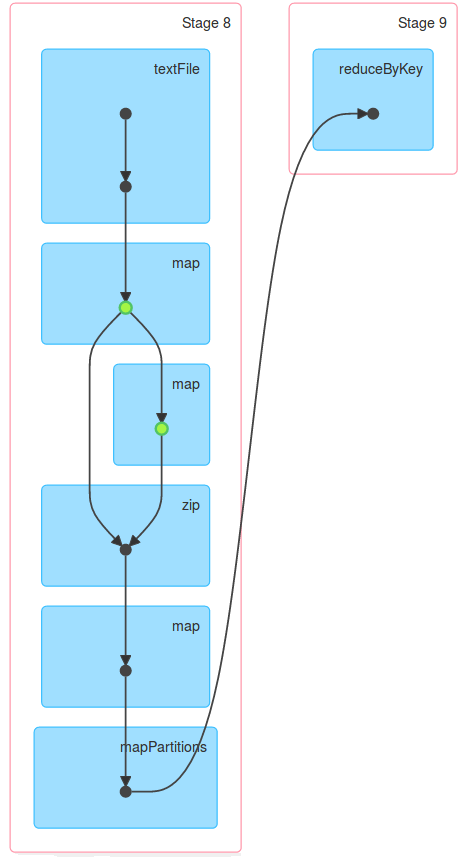
\includegraphics[width=.7\linewidth]{images/DAG1}
  \captionof{figure}{Iterative K-Means execution DAG}
  \label{fig:dag1}
\end{minipage}%
\begin{minipage}{.5\textwidth}
  \centering
  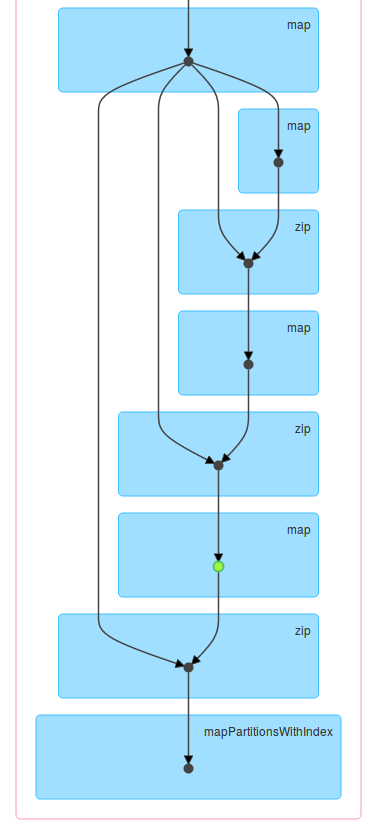
\includegraphics[width=0.6\linewidth]{images/DAG2}
  \captionof{figure}{K-Means++ execution DAG \\(the start of the DAG is identical to Iterative K-Means)}
  \label{fig:dag2}
\end{minipage}
\end{figure}

\section{Implementation of Mini-batch K-Means Clustering}

Mini-batch K-Means or Streaming K-Means (as called in MLlib) aims to overcome the limitations of Standard K-Means in regards to storage, and provides the means to do real time data processing on live sources. It is an algorithm of particular interest, as its implementation is not only reliant on the core RDD based API of Spark, but it also utilizes Spark Streaming.

Because Mini-batch K-Means does not function by performing multiple passes on the entirety of the data, it is only required that one mini-batch from the whole data is available when the new value of the cluster centers is computed for each iteration. This relieves the user from having to store the entirety of available data to execute the algorithm. The notion that only a small chunk of the data is needed at any one time can be further abstracted to the idea that the entirety of the data has not even been created yet, and that the latest acquired piece is simply a partial output of a live data producing source.

For this reason Mini-batch K-Means was seen as a good example for implementing a machine learning algorithm that trains using real time data, obtained through Spark Streaming. A Spark application would monitor a stream (with data formated as N-dimensional data points) and between a specified time interval, collect all of the newly arrived points and process them as a single mini-batch.

\subsection{API details}

As was the case with Iterative K-Means the user exposed API of Streaming K-Means is fairly simple, however, there are a several notable differences that arise from the use of streams. Firstly, as opposed to simply calling a \texttt{train()} method and receiving a \texttt{KMeansModel} object, one needs to instantiate a \texttt{StreamingKMeans} object and then call a series of mutator methods to provide the input parameters to the algorithm and establish the initial state of the \texttt{K} centroids. These methods include:

\begin{itemize}
\item \texttt{setK()}: sets the number of cluster center
\item \texttt{setDecayFactor()}: sets the forgetfulness of centroids
\item \texttt{setHalfLife()}: sets the decay factor of centroids to $\exp(log(0.5) / halflife)$
\item \texttt{setInitialCenters()}: allows the user to manually enter the initial values for the \texttt{K} centers along with their staring weights - good to use if there are strong indications of what the data distribution will be like or if the user has a previously trained model that they would like to place in a streaming environment
\item \texttt{setRandomCenters()}: allows the user to specify specify the dimensions of the \texttt{K} centers, along with their starting weights and a seed. These parameters will be used to assign random initial centroids
\end{itemize}

The two alternatives for assigning the initial values of the \texttt{K} centroids are of particular interest. In contrast with the the implementation for standard K-Means there is no option to set the initial values of the centroids to randomly selected points from the input set, or to run any centroid selection algorithm. This could be because the developers assume that the data available in the first encountered mini-batch could be either too small or unrepresentative of the expected distribution of points as time progresses. In fact the option to set a large starting weight for the initial centroids can be used to mitigate the effect of poorly distributed initial mini-batches.

Once all initialization has been completed, the algorithm can start executing by calling the \texttt{trainOn()} method and supplying an input discretized stream (\texttt{DStream}) of \texttt{Vector} objects. This method's implementation is to simply call the centroid updating algorithm for every RDD (mini-batch) produced by the DStream. After a certain amount of time has passed, or the stream has for some reasuon terminated, a user can inspect the latest value of the \texttt{K} centroids by calling the \texttt{latestModel()} method. Thus the final output of the Streaming K-Means algorithm is a \texttt{StreamingKMeansModel} object -- similar to the \texttt{KMeansModel} returned by Iterative K-Means, however, here a user also has access to the final weights attached to each centroid.

\subsection{Algorithm details}

Streaming K-Means functions primarily by making periodic updates to its \texttt{model} variable. It is an object of type \texttt{StreamingKMeansModel} -- a child inheriting from \texttt{KMeansModel} that also includes an array of weights for each of the \texttt{K} centers, along with an \texttt{update()} method. The \texttt{update()} method is responsible for changing the values of the \texttt{model} variable by operating on a single mini-batch -- to achieve this the program makes a call to \texttt{update()} from the \texttt{trainOn()} method for each RDD obtained from the DStream.

The \texttt{update()} function, invoked with an RDD of \texttt{Vector} objects, begins by using the input data to create an RDD of tuples with the following form (\texttt{closestCenterIndex}, (\texttt{originalPoint}, \texttt{1})). It then defines a \texttt{mergeContribs} function which takes two tuples of the form (\texttt{Vector}, \texttt{Long}) and produces another tuple with elements equal to the sum of the respective elements in the input tuples. The \texttt{aggregateByKey()} transformation is then invoked on the RDD of tuples with a (\texttt{tvectorOfZeroes}, \texttt{0}) tuple as a starting value for each aggregated group and the \texttt{mergeContibs} function as a combining operation. This in effect sums the value of all points ``attached'' to a particular centroid and counts how many there are. Before changing the values of the existing centroids, however, a discount is applied to the weights array, allowing the algorithm to diminish the impact of old observations.

Using the produced array of \texttt{K} tuples, each centroid corresponding to a tuple is updated as follows:

\begin{center}
\begin{BVerbatim}
lambda = numberOfSummedPoints / currentCentroidrWeight
contributionVector = contributionVector * lambda
currentCentroid = currentCentroid * (currentCentroidWeight - 1)
cuccentCentroid = currentCentroid + contibutionVector
\end{BVerbatim}
\end{center}

As a final step the algorithm computes whether the cluster center with smallest weight is dying -- i.e. its weight is more than $10^8$ time smaller than the weight the the largest cluster. If this is the case the largest cluster is split in two and the centroid of the smallest cluster is destroyed.

\begin{figure}[H]
\centering
\begin{minipage}{.5\textwidth}
  \centering
  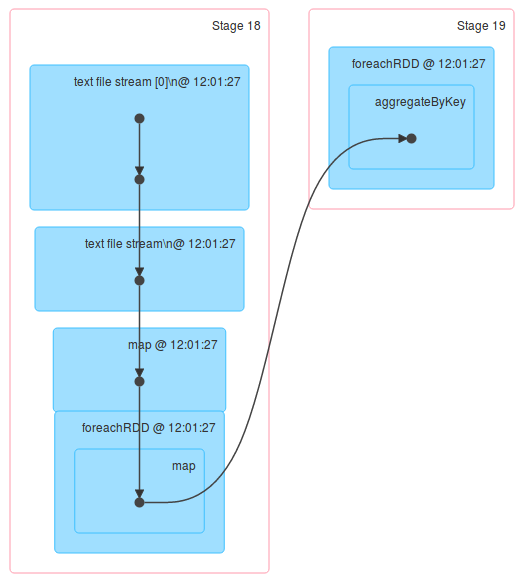
\includegraphics[width=.75\linewidth]{images/DAG3}
  \captionof{figure}{Streaming K-Means execution DAG}
  \label{fig:dag3}
\end{minipage}%
\begin{minipage}{.5\textwidth}
  \centering
  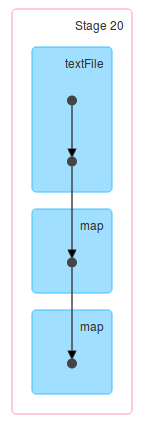
\includegraphics[width=0.29\linewidth]{images/DAG4}
  \captionof{figure}{KMeansModel computing WCSS DAG}
  \label{fig:gag4}
\end{minipage}
\end{figure}

%==============================================================================

\chapter{Proposed Extension to Spark/MLlib}
\label{propose}

One of the main drawbacks of the Iterative (standard) K-Means algorithm is its reliance on  multiple passes over a the entirety of observed data. It does this in an attempt to minimize the Within-Cluster Sum of Squares (WCSS) value -- i.e. the loss of the resulting model of \texttt{K} centroids, however, it is also prone to get stuck in local maximums. Therefore its execution has the potential to incur a massive performance overhead, while offering little in added quality.

This paper covers a variety of possible alternative \textit{Online} clustering algorithms that, through performing a single pass over the provided data, can produce models that sacrifice little in terms of quality, but offer a substantial boost in performance. Certain approaches can overcome additional limitations of Standard K-Means, such as having to manually select a value for \texttt{K} without knowing how many logical centers the data might contain. These algorithms will first be examined from a mathematical perspective.

\section{Online K-Means}

One of the most basic forms of clustering that rely on a single pass of the observed data is Lloyd's Online K-Means algorithm. As is the case with the previously discussed algorithms, Online K-Means is a competitive learning algorithm, where, for each point belonging to a given input set, the \texttt{K} centroids compete to have that point ``attach'' to them -- the winner being decided based on which centroid is closest at the time the point is being considered\cite{MLIntro}. All of this serves to reduce the WCSS value.

A distinct aspect of Online clustering algorithms that is exemplified by Lloyd's Online algorithm is how every observed point has an immediate impact on its closest centroid. In the previous case of Iterative K-Means, the closest center for each observed point is calculated without making adjustments to the locations of the centroids, which are later resigned to the average of all observed points that belong to the cluster they define. Here, upon encountering an input point and calculating which cluster it should belong to, the centroid of that cluster is immediately moved in the direction of the observed point, before considering the next one.

The amount of change a ``winning'' centroid experiences when encountering a new point is determined by the learning rate -- often depicted as $\mu$. In the original version of Lloyd's algorithm, the learning rate is expressed as the reciprocal of the number of points that had previously ``attached'' to a given centroid -- the wight of that centroid. 

\begin{center}
\begin{BVerbatim}
newCenter = oldCenter + learningRate * (observedPoint - oldCenter)
\end{BVerbatim}
\end{center}

It is clear to see that with with a learning rate of 0, the center value would not change at all, and with a learning rate on 1, the new value of the center is the same as the observed point (i.e. 100\% of the value of that center is learned from the most recent point). Therefore, because Lloyd defines learning rate as 1/\textit{centerWeight}, as our input stream of data continues, each new encountered point will have a smaller and smaller impact on its closest centroid.

A possible alternative is to set the learning rate to a constant in the range $\in$ (0,1). This approach allows the algorithm to gradually forget the effects of older observed points, which lets it adjust better to the most recently formed logical centers.

\begin{figure}[H]
	\centering
    \label{onlineGraph}
    \includegraphics[width=0.65\textwidth]{images/Graph1}
    \caption{The empty circles are the centers and the black circle is an observed point. Online K-Means moves the closest center towards the direction of ($x-c_i$) by a factor of $\mu$} 
\end{figure}

It is also important to note that Online K-Means is quite sensitive to the initial values of the \texttt{K} centroids. Because of its method of operation, if the centroids were cerated with poor starting values (e.g. two of the centroids being fairly close to one another), the final result could differ based on the order in which the points were observed.

\begin{algorithm}
\caption{Online K-Means}\label{online-alg}
\begin{algorithmic}[1]
\State Given: \textit{k}, data set \textit{X}
\State Initialize each \textbf{c} $\in$ \textit{C} with an \textbf{x} picked randomly from \textit{X}
\State Initialize counters $n_{1}, n_{2} ... n_{k}$ with a zero value
\For {\textit{x} $\in$ \textit{X}}
    \State \textbf{i}  $\gets$ \textit{getclosestCenterIndex}(\textit{C},x)
    \State \textbf{z}  $\gets$ C[i] \hspace{2.25cm} // Get the closest center
    \State n[i] $\gets$ n[i] + 1 \hspace{1.3cm} // Update the number of point in this cluster
    \State \textbf{z} $\gets$ z + $\frac{1}{n[i]}$ * (x - z) \hspace{0.35cm} // Update the cluster center
\EndFor
\State \textbf{end for}
\end{algorithmic}
\end{algorithm}

\section{Adaptive Resonance Theory K-Means}

In all of the clustering algorithms looked at so far a user specified value of \texttt{K} needed to be provided, before processing the available data. An expensive operation to determine a suitable \texttt{K} would be to run such an algorithm multiple times with different values of \texttt{K} and compare the resulting WCSS values of output models. This method, however, is not entirely reliable as the algorithm's intent is to find logical groups within the data, where as the value of WCSS (the loss of the produced model) will keep decreasing as \texttt{K} increases, and there is no clear indicator for when to stop\cite{LearnK}.

An alternative approach would be to incrementally discover a suitable value for \texttt{K} -- i.e. start with a single centroid and add more as they are needed. The Adaptive Resonance Theory (ART) algorithm\cite{ART} is one such example. In the case of ART, instead of requiring a set value for how many centroids will be trained, the algorithm takes as input a threshold value called a \textit{vigilance} (specifying a Euclidean distance in this case). 

Thus ART K-Means begins by assigning a single centroid to have the same initial value as a point, randomly selected from the input set. Then, for each new processed point, the nearest available centroid is identified (there will be only one at the start). If the distance between the observation and its closest centroid is less than the specified vigilance, the respective cluster center will be updated in the same manner as Online K-Means (Algorithm \ref{online-alg}). If the distance is greater than the vigilance, however, an new centroid is created at the location of the examined point.

\begin{figure}[H]
	\centering
    \label{artGraph}
    \includegraphics[width=0.65\textwidth]{images/Graph2}
    \caption{The distance from $x^a$ to the closest center is less than the vigilance $\rho$ -- the center is updated in the same way as Online K-Means. $X^b$ is not close enough to any of the centers and so a new centroid should be created at its position.} 
\end{figure}

The \textit{vigilance} value used in ART K-Means effectively defines a hypersphere around each centroid. Therefore, any new point that does not fall within the boundaries of an existing hypersphere creates a new one. This results in the partitioning of the examined N-dimensional space and sets a clear boundary for the region occupied by any given cluster. 

\begin{algorithm}[H]
\caption{ART K-Means}\label{art-alg}
\begin{algorithmic}[1]
\State Given: a vigilance value $\rho$, data set \textit{X}
\State Initialize one \textbf{c} $\in$ \textit{C} with an \textbf{x} picked randomly from \textit{X}
\State Initialize a single counter $n_{1}$ with a value of zero
\For {\textit{x} $\in$ \textit{X}}
    \State \textbf{i}  $\gets$ \textit{getclosestCenterIndex}(\textit{C},x)
    \State \textbf{z}  $\gets$ C[i] \hspace{2.35cm} // Get the closest center
    \State \textbf{d} $\gets$ \textit{getDistance(x, z)} \hspace{0.3cm} // Get the distance between the point and its nearest center
    \If {$d < \rho$}
        \State n[i] $\gets$ n[i] + 1 \hspace{1.3cm} // Update the number of point in this cluster
        \State \textbf{z} $\gets$ z + $\frac{1}{n[i]}$ * (x - z) \hspace{0.35cm} // Update the cluster center
    \Else
        \State \textit{C} $\gets$ \textit{C} + \textit{x} \hspace{0.55cm} // Create a new center with a value equal to the observed point
        \State $n_k$ $\gets$ 1 \hspace{1cm} // Create a counter for the new center with a weight of one
    \EndIf
\EndFor
\State \textbf{end for}
\end{algorithmic}
\end{algorithm}

ART K-Means does not entirely solve the issue of specifying an initial number of centroids but rather shifts the problem to choosing an optimal \textit{vigilance} value. Because it is possible to identify the extremes of any of the dimensions of the input points, however, one can adjust the vigilance to partition the observed space into a set number of equally sized hyperspheres. This overcomes a different weakness of traditional clustering algorithms, where the initial values of the \texttt{K} centroids could be insufficiently dissimilar (e.g. two centroids starting off at nearly identical coordinates).

\section{Self-Organizing Maps K-Means}

\section{Benefits of Online Algorithms}

\section{Implementation Challenge in Parallelizing Sequential Algorithms}

%==============================================================================

\chapter{Online K-Means}
\label{online}

\section{Implementation Using Grand Mean}

% TODO: write about first center combiner its problems and the solution

\section{Implementation using Spark Streaming}

%==============================================================================

\chapter{Adaptive Resonance Theory K-Means}
\label{art}

\section{Implementation Using Spark Streaming}

% TODO: talk about normalization of space 
% TODO: write about first center combiner its problems and the solution
% TODO: graphs of extra centers made between partitions
% TODO: picture of full space vs unit hypercube
% TODO: algorithm of combining centers

%==============================================================================

\chapter{Self-Organizing Maps K-Means}
\label{som}

\section{Implementation Using Spark Streaming}

%==============================================================================

\chapter{Performance Evaluation and Data Model Analysis}
\label{eval}

% TODO: maybe add an evaluation section earlier to each part\\
% add chapter comparing algorithms at the end\\
% both would need to explain evaluation method earlier\\
% make a reference to the used training data

% TODO: talk about silhouette - include pseudo code and picture 

\section{Sum of Squared Distances}

\section{Silhouette}

%==============================================================================

\chapter{Conclusion}
\label{conclusion}

% TODO: conclusion text - multiple sections?

%==============================================================================

\bibliographystyle{plain}
\bibliography{l4proj}

%==============================================================================

\begin{appendices}

\chapter{First Appendix}

\end{appendices}

\end{document}
